\newpage
\section{Exercise 2-4}
To investigate driven oscillations a electric motor is used to drive the oscillation.
The position of the flywheel is again determined by the CASSY system and recorded
on the PC. To get the data for exercise 3 and 4 also the phase shift and the 
transient responses are observed qualitively. Over the whole task the damping constant
\(\delta_1\) was used.

\subsection{Observation}

\subsubsection{Exercise 2}
To determine the amplitude \(A\) as a function of the drive frequency \(\Omega\) 
the interval of drive frequencies is chosen so that it contains the resonance frequency 
\(\omega_1\) and the values near the resonance frequency. The amplitude has a exponential decreasing envelope
function and so it is nescesery to wait until the amplitude is almost constant. The
frequncies are determined by just counting the periods per time interval.
  
\subsubsection{Exercise 3}
It is very clear that in this experiment the observes phase shift qualitively absolutely fits
with the theoretical function. For very small \(\Omega\) the phase shift is \(\phi
= 0\) for high frequencies the phase shift is \(\phi = - \pi\) and near the resonance
frequency it is \(\phi = -\pi/2 \).

\subsubsection{Exercise 4}
The behavior of the transient responses also fits with the theory. In the case that
the drive frequency is almost the resonance frequency the amplitude just grows until
it gets constant. Otherwise the amplitude has ha exponetial decreasing swing behavior. 

\subsection{Measured Data}
\begin{center}
\begin{tabular}{c|c|c|c|c|c}
\(t_1 [s]\) & \(t_2 [s]\) & \(N\) & \(\omega_1 [1/s]\) & \(A \propto [m]\) \\\hline
\(234.18\) & \(267.84\) & \(15\) & \(0.445632798573976\) & \(0.56\) \\ 
\(51.28\) & \(92.48\) & \(20\) & \(0.485436893203883\) & \(0.1\) \\ 
\(136.16\) & \(97.34\) & \(20\) & \(0.515198351365276\) & \(0.27\) \\ 
\(114.8\) & \(153.16\) & \(20\) & \(0.521376433785193\) & \(0.36\) \\ 
\(151.88\) & \(113.6\) & \(20\) & \(0.522466039707419\) & \(0.4\) \\ 
\(146.72\) & \(108.66\) & \(20\) & \(0.525486074619022\) & \(0.56\) \\ 
\(290.62\) & \(253.02\) & \(20\) & \(0.531914893617021\) & \(0.73\) \\ 
\(215.58\) & \(178.56\) & \(20\) & \(0.540248514316586\) & \(0.35\) \\ 
\(541.33\) & \(539.45\) & \(1\) & \(0.531914893617023\) & \(0.76\) \\ 
\(215.12\) & \(189.36\) & \(20\) & \(0.77639751552795\) & \(0.24\) \\ 
\(128.08\) & \(164.7\) & \(20\) & \(0.546149645002731\) & \(0.27\) \\ 
\(160.42\) & \(123.24\) & \(20\) & \(0.537923614846692\) & \(0.4\) \\
\end{tabular}
\end{center}

\subsection{Errors}
The Error will be determined by the variance of the values so the errors of the measured
data have no relevance and wont be determined.

\subsection{Evaluation}
To determine the resonance frequency \(\omega_1\) and the damping constant \(\delta\)
it is assumed that the theory is correct and the dependence of \(A(\Omega)\) is correct.
That means that a fitting function in the form 
\begin{align}
f(x)=\frac{a}{\sqrt((b^2-x^2)^2+4(cx)^2)}
\end{align}
is used. In comparison to \eqref{A(W)} it is clear that
\begin{align}
a &= \frac{F_0}{m} \\
b &= \omega_1 \\
c &= \delta
\end{align}

\subsubsection{Graphs}
To have a first look at the values they are plotted:
\begin{center}
\begin{minipage}{\linewidth}
\centering
\makebox[0cm]{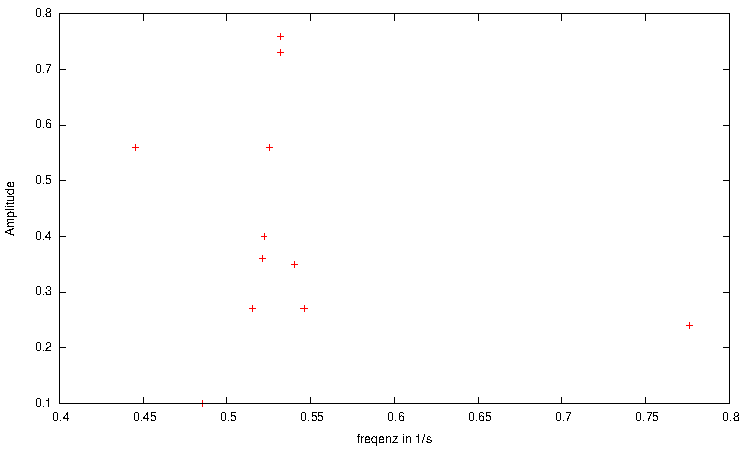
\includegraphics[width=\textwidth]{graphen/a2'}}
\end{minipage}
\captionof{figure}{plotted measure values}
\end{center}
It is clear that two values don't represent a continous function. It is quite likely that at the measuring of 
those two values something went wrong. They are just rejected to get a continous function.
\begin{center}
\begin{minipage}{\linewidth}
\centering
\makebox[0cm]{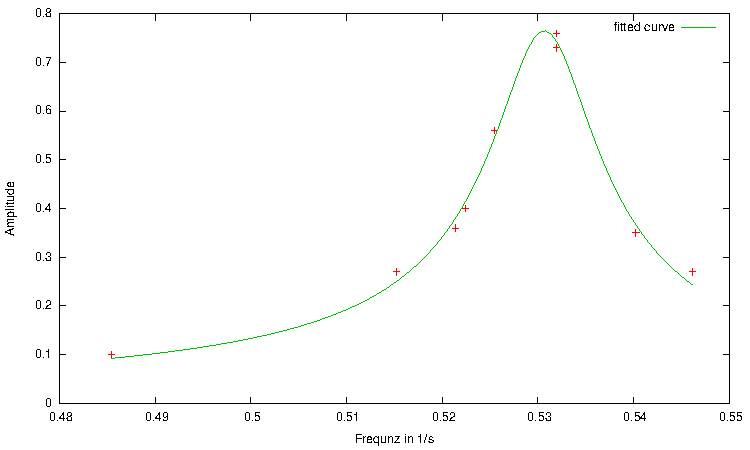
\includegraphics[width=\textwidth]{graphen/a2}}
\end{minipage}
\captionof{figure}{reduced plotted measure values with fitting curve}
\end{center}
The parameters are determined to:
\begin{align}
a &= (0.00428 \pm 0.00017) \, m/s^2 \notag \\
b &= (0.53073 \pm 0.00029) \, 1/s \notag \\
c &= (0.03514 \pm 0.00028) \, 1/s \notag
\end{align}
So the eigenfrequency and the damping constant are:
\begin{align}
\omega_1 &= (0.53073 \pm 0.00029) \, 1/s \notag \\
\delta_1 &= (0.03514 \pm 0.00086) \, 1/s \notag
\end{align}
\subsection{Summary}
The final result for the Values is:
\begin{align}
\omega_1 &= (0.5307 \pm 0.0003) \, 1/s \notag \\
\delta_1 &= (0.0351 \pm 0.0009) \, 1/s \notag
\end{align}
which is almost the same as determined in exercise 1.
